\documentclass[tikz,border=0pt]{standalone}
\usepackage[T1]{fontenc}
\usepackage{helvet}
\renewcommand{\familydefault}{\sfdefault}
\usepackage{xcolor}
\usetikzlibrary{arrows.meta}

\definecolor{nvidiagreen}{HTML}{76B900}
\definecolor{nvgray}{HTML}{767676}
\definecolor{nvcharcoal}{HTML}{4D4D4D}
\definecolor{nvblack}{HTML}{333333}

\newcommand{\Stage}[6]{%
  \node[font=\bfseries\fontsize{24}{28}\selectfont,text=nvblack,align=center]
    at (#1,4.25) {#2};
  \node[font=\ttfamily\fontsize{10}{12}\selectfont,text=nvgray,align=center]
    at (#1,3.90) {#3};
  \node[font=\fontsize{15}{18}\selectfont,text=nvcharcoal,align=center]
    at (#1,3.18) {#4};
  \node[font=\bfseries\fontsize{11}{13}\selectfont,text=nvidiagreen,align=center]
    at (#1,2.25) {#5};
  \node[font=\fontsize{11}{13}\selectfont,text=nvgray,align=center]
    at (#1,1.98) {#6};
}

\begin{document}
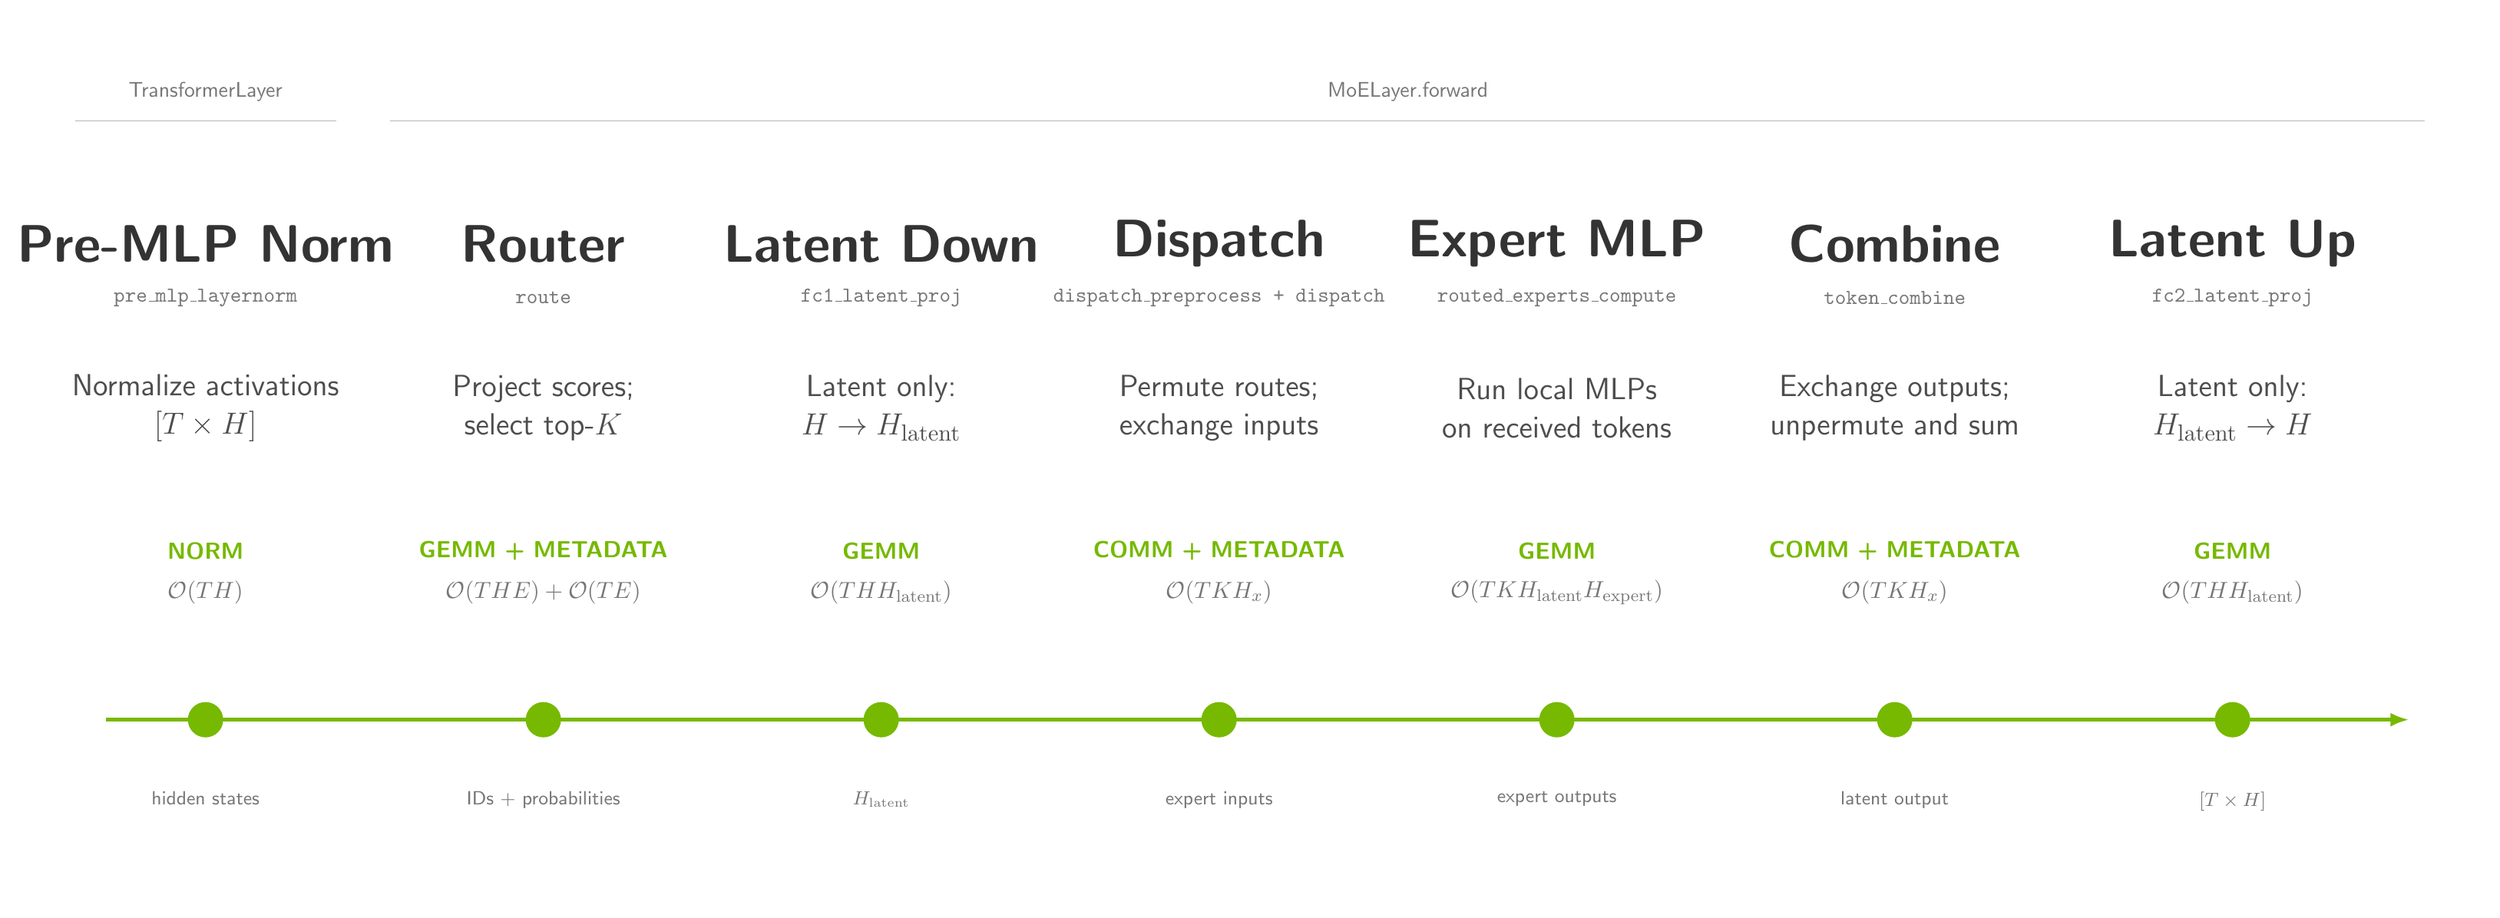
\begin{tikzpicture}[x=1in,y=1in]
  \path[use as bounding box] (0,0) rectangle (16,5.7);

  \draw[nvgray!55,line width=.45pt] (.35,5.05) -- (2.05,5.05);
  \node[font=\fontsize{10}{12}\selectfont,text=nvgray,anchor=south]
    at (1.20,5.13) {TransformerLayer};
  \draw[nvgray!55,line width=.45pt] (2.40,5.05) -- (15.65,5.05);
  \node[font=\fontsize{10}{12}\selectfont,text=nvgray,anchor=south]
    at (9.03,5.13) {MoELayer.forward};

  \Stage{1.20}{Pre-MLP Norm}{pre\_mlp\_layernorm}
    {Normalize activations\\$[T \times H]$}{NORM}{$\mathcal{O}(T H)$}
  \Stage{3.40}{Router}{route}
    {Project scores;\\select top-$K$}{GEMM + METADATA}{$\mathcal{O}(T H E) + \mathcal{O}(T E)$}
  \Stage{5.60}{Latent Down}{fc1\_latent\_proj}
    {Latent only:\\$H \rightarrow H_{\mathrm{latent}}$}{GEMM}{$\mathcal{O}(T H H_{\mathrm{latent}})$}
  \Stage{7.80}{Dispatch}{dispatch\_preprocess + dispatch}
    {Permute routes;\\exchange inputs}{COMM + METADATA}{$\mathcal{O}(T K H_x)$}
  \Stage{10.00}{Expert MLP}{routed\_experts\_compute}
    {Run local MLPs\\on received tokens}{GEMM}{$\mathcal{O}(T K H_{\mathrm{latent}} H_{\mathrm{expert}})$}
  \Stage{12.20}{Combine}{token\_combine}
    {Exchange outputs;\\unpermute and sum}{COMM + METADATA}{$\mathcal{O}(T K H_x)$}
  \Stage{14.40}{Latent Up}{fc2\_latent\_proj}
    {Latent only:\\$H_{\mathrm{latent}} \rightarrow H$}{GEMM}{$\mathcal{O}(T H H_{\mathrm{latent}})$}

  \draw[-{Latex[length=3.1mm]},nvidiagreen,line width=1.8pt] (.55,1.15) -- (15.55,1.15);
  \foreach \x in {1.20,3.40,5.60,7.80,10.00,12.20,14.40}
    \fill[nvidiagreen] (\x,1.15) circle (.115);
  \node[font=\fontsize{9}{11}\selectfont,text=nvgray,anchor=north] at (1.20,.73) {hidden states};
  \node[font=\fontsize{9}{11}\selectfont,text=nvgray,anchor=north] at (3.40,.73) {IDs + probabilities};
  \node[font=\fontsize{9}{11}\selectfont,text=nvgray,anchor=north] at (5.60,.73) {$H_{\mathrm{latent}}$};
  \node[font=\fontsize{9}{11}\selectfont,text=nvgray,anchor=north] at (7.80,.73) {expert inputs};
  \node[font=\fontsize{9}{11}\selectfont,text=nvgray,anchor=north] at (10.00,.73) {expert outputs};
  \node[font=\fontsize{9}{11}\selectfont,text=nvgray,anchor=north] at (12.20,.73) {latent output};
  \node[font=\fontsize{9}{11}\selectfont,text=nvgray,anchor=north] at (14.40,.73) {$[T \times H]$};
\end{tikzpicture}
\end{document}
